\section{Gradient Descent}
If you have spent more than an hour (or in some cases, a second) with someone involved in Computer Science (or increasingly, STEM in general) you have probably heard of gradient descent. The elevator pitch of the method is essentially ``start with a guess, and then move in the direction of steepest decrease''. Recall from multivariable calculus (or physics) that the negative gradient is the direction of steepest descent, hence the name. In this section we will first try to somewhat motivate the utility of gradient descent (as opposed to other optimization methods), and then take a gander at what it looks like in different settings. In particular, we will look at the various variants of GD, and analyze their performance in different settings.

\subsection{Least Squares problems}
\subsubsection{Motivation and Setup}
A simple way to build any sort of predictive model is to conjecture some form of a ``feature basis'', and then try to find the best fit of the data to this basis. For instance, we might want to find the best fit cubic polynomial, or combination of sine/cosine waves, or even just a best-fit linear model. In each case, it's a matter of finding the coefficients $\inn{c_1, \dots, c_k}$ which results in our resultant function's evaluation on the training points match the expected output.

More formally, we may define a matrix $\A \in \R^{n \times d}$ such that
\begin{align*}
    \A_{ij} = \varphi_i\left(x^{(j)}_i\right)
\end{align*}
where $\inn{\varphi_1, \dots, \varphi_d}$ defines our feature basis. Then, our task is to solve
\begin{align*}
    \A\bx = {\bf b}
\end{align*}
where $\bx$ is our vector of coefficients. We will generally consider the case where this system is overdetermined. i.e., where we have more training samples than coeffecients $(n > d)$. In a practical setting, it is more feasible to instead look for an approximate solution $\bx$ simply satisfying $\A\bx \approx {\bf b}$.

One way to do it is to find $\bx$ which minimizes some measure of ``badness''. We shall now refer to this measure as a ``loss function'', denoted as $\L$. Thus, we want to find
\begin{align*}
    \min_{\bx \in \R^d} \L(\A, \bx, {\bf b})
\end{align*}
It remains to determine what $\L$ is. Intuitively, $\L$ should certainly involve the error $\A\bx - {\bf b}$. We could pick
\begin{align*}
    \L(\A, \bx, {\bf b}) = \norm{\A\bx - {\bf b}}_0
\end{align*}
where $\norm{u}_0 = |\mathrm{supp}(u)|$ is the number of non-zero entries in a vector. Intuitively, this is trying to find the ``simplest'' solution, as a proxy for generalization (along the lines of Occam's razor). However, this is a combinatorially hard problem, and thus perhaps not a great idea. What about
\begin{align*}
    \L(\A, \bx, {\bf b}) = \norm{\A\bx - {\bf b}}_1
\end{align*}
Well, minimizing the $1$-norm is at some level a proxy for minimizing the $0$-norm so it's a good idea in that sense. However, it is not differentiable everywhere. Differentiability is in general a good property to have, as it makes the problem amenable to various optimization techniques. What about the $2$-norm?
\begin{align*}
    \L(\A, \bx, {\bf b}) = \norm{\A\bx - {\bf b}}_2^2
\end{align*}
You might have noticed I sneaked in a square in there. As it turns out, the $2$-norm is somehow the Goldilocks zone of norms (see Scott Aaronson's lecture notes on Quantum Information Science \cite{aaronson_2018} for a similar observation in that realm). This loss function is twice-differentiable everywhere, and {\em convex} (see \autoref{sec:convex}). As we will see soon, this means our problem has a unique solution, and moreover has a nice closed form.

    \subsubsection{Solving Least Squares}
        The problem we want to solve can now be written out as
        \begin{align*}
            \min_x \norm{\A\bx - {\bf b}}_2^2 = \min_x \sum_{i=1}^n \lp \inn{\A_{i, \bullet}, \bx} - b_i\rp^2 = \min_{x_1, \dots, x_d} \sum_{i =1}^n \lp \sum_{j = 1}^d \A_{ij}\bx_j - b_i \rp^2
        \end{align*}
        We let our loss function be $\L(x) = \half \norm{\A\bx - {\bf b}}_2^2$. Then, to minimize we solve for the stationary points of $\L$. However, since $\L$ is convex, this will also be the global minimizer!
        \begin{align*}
            \frac{\partial \L}{\partial \bx_j} = \frac{\partial}{\partial \bx_j} \half \sum_{i = 1}^n \lp \inn{\A_{i, \bullet}, \bx} - b_i \rp^2 
            = \sum_{i = 1}^n \lp \inn{\A_{i, \bullet}, \bx} - b_i \rp \frac{\partial}{\partial \bx_j} \lp \inn{\A_{i, \bullet}, \bx} - b_i \rp \\
            =  \sum_{i = 1}^n \A_{ij} \lp \inn{\A_{i, \bullet}, \bx} - b_i \rp = \inn{\lp \A_{1j}, \dots, \A_{nj} \rp, \A\bx - {\bf b}} \\ = \inn{\A_{\bullet, j}, \A\bx - {\bf b}}
        \end{align*}
        Thus, we have that the gradient $\grad \L$ satisfies
        \begin{equation}
        \label{eqn:leastsq:grad}
            \grad \L := \lp \frac{\partial \L}{\partial \bx_j}\rp_{j = 1}^d = \A^\top(\A\bx - {\bf b})
        \end{equation}
        Thus, solving for the stationary points,
        \begin{align*}
            \grad \L = 0 \\
            \iff \A^\top (\A\bx - {\bf b}) = 0 \iff \A^\top \A\bx = \A^\top {\bf b} \\
            \iff \boxed{\bx = (\A^\top \A)^{-1} \A^\top {\bf b}}
        \end{align*}
        The term $(\A \A^\top)^{-1}\A^\top$ is also known as the {\em Moore-Penrose psuedoinverse}.
        \begin{defn}[Moore-Penrose psuedoinverse]
        For a full-rank overdetermined matrix $\A \in \R^{n \times d}$, the matrix $\A^\dagger := (\A^\top \A)^{-1}\A^\top \in \R^{d \times n}$ is call the (Moore-Penrose) psuedoinverse of $\A$.
        \begin{enumerate}
            \item $\A^\dagger$ is a {\em left} inverse of $\A$. That is, $\A^\dagger \A = \I_{d \times d}$.
            \item The psuedoinverse $x^* = \A^\dagger$ is the solution to the linear least squares problem.
        \end{enumerate}
        \end{defn}
        \paragraph{Properties of the Psuedoinverse}
        The psuedoinverse also has the following interesting properties:
        \begin{prop}
        $\A\A^\dagger \in \R^{n \times n}$ is an {\rm orthogonal projection matrix} onto the subspace spanned by the columns of $\A$. Similarly $(\A\A^\dagger - \I)$ is an orthogonal projection onto the complementary space.
        \end{prop}
        \begin{prop}
        The vector $\A\bx^* = \A\A^\dagger {\bf b} \in \R^n$ minimizing the least squares loss is the projection of ${\bf b}$ onto the subspace $\A\A^\dagger$ spanned by the columns of $\A$.
        \end{prop}
        \subsubsection{Least Squares Example}
        A simple instance of least squares is finding the best linear fit to a data set. i.e., find the best line $mx + b$ minimizing the sum of squared {\em vertical} offsets
        \begin{align*}
            \min_{m,b} \sum_{i = 1}^n \lp mx_i + b - y_i\rp^2
        \end{align*}
        In matrix form,
        \begin{align*}
            \min_{m,b} \norm{\A \begin{pmatrix}m & b \end{pmatrix}^\top - {\bf y}}_2^2
        \end{align*}
        where
        \begin{align*}
            \A = \begin{pmatrix}
            x_1 & 1 \\
            x_2 & 1 \\
            \vdots & \\
            x_n & 1
            \end{pmatrix}
        \end{align*}
        The least squares solution can then be calculated as follows:
        \begin{align*}
            \begin{pmatrix}
                    m^* \\
                    b^*
            \end{pmatrix} = (\A^\top \A)^{-1} \A^\top {\bf y} \\
            m^* =
                    \frac{\sum_{i = 1}^n x_iy_i}{\sum_{i = 1}^n x_i^2} \quad  b^* = 
                    \frac{1}{n} \sum_{i = 1}^n y_i
        \end{align*}
        \subsubsection{Efficiency of Solving Least Squares}
        Solving the least squares problem using the above psuedoinverse method is quite inefficient, since just to compute a single vector $\bx^*$ we need to invert a large matrix which can be a very expensive operation. While it is true that as we saw above the unique solution $\bx^*$ can be obtained by solving the linear system
        \begin{align*}
            \A^\top \A \bx^* = \A^\top {\bf b}
        \end{align*}
        with highly specialized linear solvers, we are more interested in general iterative solvers that extend beyond simple linear models. This is where \textbf{gradient descent} comes in.
        
        \subsubsection{Solving Least Squares with Gradient Descent}
        Gradient Descent is an extremely general, and simple first-order optimization method. The key intuition/insight is that in order to minimize a function, we keep moving in the direction of the negative gradient. The reader may recall that this is the direction of steepest decrease.
        \begin{algorithm}[H]
        \caption{Gradient Descent Psuedocode}
        \label{algo:gd}
        \begin{algorithmic}[1]
        \Procedure{GradientDescent}{$f, \eta$}
        \State Initialize $x_0 \in_R \R^d$
        \While{not converged}
            \State $x_{t+1} = x_t - \eta \grad f(x_t)$
        \EndWhile
        \Return $x_{t+1}$
        \EndProcedure
        \end{algorithmic}
        \end{algorithm}
        Now, specifically for the case of linear least squares, we recall \autoref{eqn:leastsq:grad}
        \begin{align*}
            \grad \L = \A^\top (\A\bx - {\bf b})
        \end{align*}
        Thus, the least squares gradient descent update becomes
              \begin{algorithm}
        \label{algo:leastsq:gd}
        \caption{Linear Least Squares Gradient Descent}
        \begin{algorithmic}[1]
        \Procedure{LinearLeastSquaresGD}{$\A, {\bf b}, \eta$}
        \State Initialize $x_0 \in_R \R^d$
        \While{not converged}
            \State $x_{t+1} = x_t - \eta \A^\top (\A\bx - {\bf b})$
        \EndWhile
        \Return $x_{t+1}$
        \EndProcedure
        \end{algorithmic}
        \end{algorithm}
        
    \subsubsection{Convergence of Gradient Descent}
    Although we have this seemingly wonderful iterative algorithm, it is imperative that we also establish bounds on how long it will take for it to converge given some convergence criterion. If, for instance, it takes $\O(2^n)$ rounds, that's kind of useless. Well, thankfully as it turns out GD isn't useless, and in fact we can prove the following convergence guarantee:
\begin{mdframed}
    \begin{theorem}
        For the linear least squares problem, the gradient descent algorithm can meet the following convergence criterion in $\O(\log \epsilon)$ iterations, for any $\epsilon > 0$:
        \begin{align*}
            \norm{\bx_{t+1} - \bx^*}_2 \leq \epsilon \cdot \norm{\bx_0 - \bx^*}_2
        \end{align*}
    \end{theorem}
\end{mdframed}    

    \begin{proof}
    We will proceed by first bounding $\norm{\bx_{t + 1} - \bx^*}$, and then proving our choice of $\eta$ implies a convergence with the desired rate. Observe
\begin{align*}
    \bx_{t+1} - \bx^* = \lp \bx_t - \eta\A^\top(\A\bx_t - {\bf b}) \rp - \bx^* \tag{GD update}\\
    = \lp \bx_t - \eta \A^\top \lp \A\bx_t - \A\bx^* \rp \rp - \bx^* \tag{$\A\bx^* = {\bf b}$ by assumption}\\
    = \bx_t - \bx^* - \eta \A^\top\A \lp \bx_t - \bx^* \rp \\
    = (\I - \eta \A^\top \A)(\bx_t - \bx^*)
\end{align*}
We will now use the following property of the operator $2$-norm (see \autoref{sec:linalg:opnorm})
\begin{prop}
    The operator norm $\norm{\cdot}_2$ on matrices is submultiplicative. i.e.,
    \begin{align*}
        \norm{\A {\bf B}}_2 \leq \norm{\A}_2 \norm{{\bf B}}_2
    \end{align*}
\end{prop}
Thus, we now obtain the following bound
\begin{align*}
    \norm{\bx_{t + 1} - \bx^*}_2 \leq \norm{\I - \eta \A^\top\A}_2 \cdot \norm{\bx_t - \bx^*}_2
\end{align*}
In order for convergence, we need this to be a decreasing series. In particular, we need $\norm{\I - \eta \A\A^\top}_2 < 1$. We now attempt to find $\eta$ so that this is satisfied.
Recall the following property of the norm:
\begin{prop}
    The operator norm $\norm{\cdot}_2$ satisfies $\norm{\A}_2 = \sigma_1$.
\end{prop}
Thus, we will now bound the largest eigenvalue of $(\I - \eta \A^\top\A)$ and then appropriately pick $\eta$ so we get a contraction.
In particular, suppose $\A^\top \A$ has eigendecomposition $\A^\top\A = {\bf U} \Lambda {\bf U}^\top$.
Then, $\I - \eta\A^\top\A$ has eigendecomposition ${\bf U} (\I - \eta\Lambda) {\bf U}^\top$ .
Hence, the eigenvalues satisfy
\begin{align*}
    1 - \eta\lambda_{\max} \leq \dots \leq 1 - \eta\lambda_{\min}
\end{align*}
Where $\lambda_{\min}, \lambda_{\max}$ are the smallest, and largest eigenvalues of $\A^\top\A$ respectively.
Thus, since $n > d$, we have that $$\norm{\I - \eta \A^\top\A}_2 \leq (1 - \eta \lambda_{\min})$$
In order for this to be a contraction, we need
\begin{align*}
    (1 - \eta\lambda_{\min{}}) < 1 \\
\end{align*}
Observe that for $\eta \leq 1/\lambda_{\max{}}$ we have $ 0 \leq \lp 1 - \eta \lambda_{\max{}} \rp \leq \lp 1 - \eta \lambda_{\min{}} \rp < 1$
\begin{align*}
    \norm{\bx_{t+1} - \bx^*}_2 \leq \lp1 - \eta \lambda_{\min} \rp \cdot \norm{\bx_t - \bx^*}_2 \\
    \leq \lp 1 - \eta \lambda_{\min} \rp^t \cdot \norm{\bx_0 - \bx^*}_2
\end{align*}
Thus we can meet the following convergence criterion for any $\epsilon > 0$ within $\O(\log \epsilon)$ iterations. The optimal rate is obtained when we pick $\eta = 1/\lambda_{\max}$.
\begin{align*}
    \norm{\bx_{t + 1} - \bx^*}_2 \leq \epsilon \cdot \norm{\bx_0 - \bx^*}_2
\end{align*}

    \end{proof}
    % \begin{corollary}
    %     For the linear least squares problem, the gradient descent algorithm has exponential convergence rate
    %       \begin{align*}
    %         \norm{\bx_{t+1} - \bx^*}_2 \leq \lp 1 - \frac{1}{\kappa(\A)} \rp^t \cdot \norm{\bx_0 - \bx^*}_2
    %     \end{align*}
    %     where
    %     \begin{align*}
    %         \kappa(\A) = \frac{\sigma_{\max}(\A)}{\sigma_{\min}(\A)}
    %     \end{align*}
    %     is the {\em condition number} of $\A \in \R^{n \times d}$, for $\eta = 1/\lambda_1$.
    % \end{corollary}
        
\subsection{Convergence of GD for Smooth Functions}
In Machine Learning in general, while model families come in different shapes and sizes -- from simple best-fit feature bases, to SVMs, to deep neural networks -- it is still a common occurence that the loss function $\L$ has a special property: smoothness.
\begin{defn}
A differnetiable function $f$ is called \textbf{smooth} iff it has a Lipschitz continuous gradient. i.e., there exists $L$ such that
\begin{align*}
    \norm{\grad f(y) - \grad f(x)}_2 \leq L \norm{y - x}_2
\end{align*}
\end{defn}
Thus, herein we shall equivalently assume that $\grad \L$ is $L$-Lipschitz for some $L$. To study the convergence of GD, we will attempt to bound $\norm{\grad \L(w_k)}^2$. In particular, we will show the following:
\begin{mdframed}
\begin{theorem}
Fix $\eta = 1/L$. Then, we will achieve stopping criterion $\norm{\grad \L(w_t)}^2 \leq \epsilon$ in at most
\begin{align*}
    t = \frac{2L[\L(w_0) - \L^*]}{\epsilon}
\end{align*}
where $\L$ is assumed to be smooth, and $L$ is the Lipschitz constant for $\grad \L$.
\end{theorem}
\end{mdframed}

In order to prove things about $\norm{\grad \L}^2$, it's a good idea to first get a bound for $\L(w)$ in terms of $\grad L$. We will utilize the following variant of the multivariate Taylor expansion:
\begin{theorem}
\label{thm:9:3}
For a $C^2$ function
\begin{align*}
    f(y) \leq f(x) + \grad f(x)^\top (y - x) + \half (y-x)^\top \grad^2f(x^*)(y - x)
\end{align*}
\end{theorem}
However, we also want to utilize our smoothness assumption on $\L$. We will make use of the following lemma:
\begin{lemma}
\label{lem:9:3:1}
For $C^2$ functions, Lipschitz continuity of the gradient is equivalent to
\begin{align*}
    \grad^2 f(w) \preccurlyeq L \cdot \I_{d\times d}
\end{align*}
    where $A \preccurlyeq B$ iff  $B - A$ is positive semidefinite. Equivalently, we have
    $v^\top \grad^2 f(w)v \leq L\norm{v}_2^2 \, \forall v,w$
\end{lemma}
We will now apply \autoref{lem:9:3:1} to \autoref{thm:9:3} to obtain the following ``Descent Lemma'':
\begin{lemma}[Descent Lemma]
For smooth $\L$, it is the case that
\begin{align*}
    \L(y) \leq \L(x) + \grad\L(x)^\top(y - x) + \frac{L}{2}\norm{y - x}^2
\end{align*}
\end{lemma}
The Descent Lemma also holds for $C^1$ functions. This lemma gives us a quadratic upper bound function for $f$, touching at $f(x)$. To get a sense of what kind of learning rate/step size we should use, it might be a good idea to look at the minimizer for this upper bound. A simple calculation shows that the minimizer is
\begin{align*}
    y - x - \frac{1}{L} \grad \L(x)
\end{align*}
i.e., one gradient step away from $x$, with learning rate $\frac{1}{L}$. Ok, so now we will pick a constant step-size $\alpha = 1/L$ as our starting point. Using this, we will be able to prove the following theorem:
\begin{mdframed}
\begin{theorem}
\label{gd:thm:smooth:convg}
Suppose that $\L$ is smooth, and we pick a step-size $\alpha = \frac{1}{L}$. Then, the following holds:
\begin{align*}
    \min_{k \in [t]}{\; \norm{\grad \L(w_k)}^2} \leq \frac{2[\L(w_0) - \L^*]}{t}
\end{align*}
\end{theorem}
\end{mdframed}

\begin{proof}
Suppose we pick $\alpha = 1/L$. Then, our gradient update is the following:
\begin{align*}
    w_{t+1} = w_t - \frac{1}{L}\grad \L(w_t)
\end{align*}
Substituting this into the ``Descent Lemma'' from \ref{lem:9:3:1} we get
\begin{align*}
    \L(w_{t+1}) \leq \L(w_t) + \grad \L(w_t)^\top \lp -\frac{1}{L} \cdot \grad \L(w_t)\rp + \frac{L}{2} \norm{\frac{1}{L} \grad \L(w_t)}^2 \\
    = \L(w_t) - \frac{1}{L}\norm{\grad\L(w_t)}^2 + \frac{1}{2L} \norm{\grad \L(w_t)}^2 \\
    = \L(w_t) - \frac{1}{2L}\norm{\grad \L(w_t)}^2 \\
    \L(w_{t+1}) \leq \L(w_t) - \frac{1}{2L}\norm{\grad\L(w_t)}^2
\end{align*}
We may rearrange this last result to get
\begin{align*}
    \norm{\grad \L(w_t)}^2 \leq 2L\left[\L(w_t) - \L(w_{t+1})\right]
\end{align*}
Finally, we sum up the squared norms of these gradients to get
\begin{align*}
    \sum_{k = 1}^t \norm{\grad L(w_t)}^2 \leq 2L \sum_{k = 1}^t\left[\L(w_k) - \L(w_{k+1})\right] 
    \leq 2L\left[\L(w_0) - \L(w_{t+1})\right] \leq 2L\left[\L(w_0) - \L^*\right]
\end{align*}
where $\L^*$ is the minimum value of $\L$. Thus, we derive our final result
\begin{align*}
        \min_{k \in [t]}{\; \norm{\grad \L(w_k)}^2} \leq \frac{2[\L(w_0) - \L^*]}{t}
\end{align*}

\paragraph{Picking $\alpha$ in practice}
It's not really a good idea to compute $L$ in order to use $\alpha = 1/L$ in practice, since computing $L$ is usually very expensive to compute. Moreover, this is a very small step-size as it is a \textbf{worst}-case bound on curvature. Generally, it is preferred to use line-search techniques.

For instance, we may decrease $\alpha$ by binary search until the following {\em Armijo condition} is met:
\begin{align*}
    f(w_t - \alpha\grad f(w_t)) \leq f(w_t) - \alpha\gamma\norm{\grad f(w_t)}^2  \quad \gamma \in (0, 1/2]
\end{align*}
\end{proof}

\subsubsection{Concluding Notes}
The cost of computing a gradient scales with the number of variables $d$. Thus, if we are working with $n$ training samples and computing a gradient, by linearity of the gradient it'll take us $\O(nd)$ time. Above, we showed that for smooth functions GD has a guaranteed $O(1/t)$ convergence rate. i.e., if we want to converge to an $\epsilon$-approximation of a stationary point, $O(1/\epsilon)$ iterations suffice. But then, including gradient computations that's at least $\O(nd/\epsilon)$ time (huge!). This, however, (thankfully?) is at least in part an artifact of this being a very loose bound. Gradient descent is {\bf much} faster in practice. However, this does not mean GD is finding {\bf global} minimizers efficiently -- $\NP$-hard functions still exist.

In order to find global optimums of non-convex smooth functions, the fastest possible algorithms require $\O(1/\epsilon^d)$ iterations in the worst case. Smoothness is too ``local'' or ``weak'' of a model to overcome the curse of dimensionality.
\begin{displayquote}
{\em ``The biggest open question in neural network theory over the past 15 years: how is it possible that gradient descent tends to converge to global minimizers of (highly nonlinear, highly nonconvex) neural network loss functions in practice, as if such optimization problems were not much more complex than linear regression? What is the underlying structure of neural networks as implemented in practice that allows us to overcome the curse of dimensionality?'' -- R. Ward}
\end{displayquote}
Convex functions, however, are able to overcome the curse. In particular, $\O(1/\epsilon)$ iterations of GD will do the trick of bringing us $\epsilon$-close to a {\bf global} optimum, since with a convex function a stationary point is a global minimizer. There are even algorithms which can achieve $\O(1/\sqrt{\epsilon})$.
\paragraph{Nesterov's accelerated gradient method}
This method achieves the aforementioned $\O(1/\sqrt{\epsilon}$ bound. Instead of a simple constant-sized step, this method uses the previous gradient as well. In particular, it makes the following update:
\begin{align*}
    w_{t+1} = v_t - \alpha \grad f\lp v_t \rp \\
    v_{t+1} = w_t + \beta_t\lp w_{t+1} - w_t \rp
\end{align*}
This method with $\alpha_t = 1/L$ and $\beta_t = \frac{t -1 }{t + 2}$ achieves an error of $\O(1/t^2)$ after $t$ iterations.

\subsection{Convergence of GD for Convex Functions, Polyak-Lojasiewic Inequality}
While smoothness alone may not have been enough to overcome the curse of high dimensionality, all hope is not lost. Notice that for some ``nice'' functions, for instance overdetermined linear regression, gradient descent has a much faster convergence rate. In particular, it converges {\bf expoenentially} fast. A general property underlying many such ``nice'' functions is the {\em Polyak-Lojasiewic (PL) Inequality}.
\begin{defn}[Polyak-Lojasiewic Inequality]
\label{gd:defn:pl}
A function $f: \R^d \to \R$ satisfies the PL inequality iff
\begin{align*}
    \half \norm{\grad f(w)}^2 \geq \mu \lp f(w) - f^* \rp
\end{align*}
\end{defn}
\begin{example}
For the least squares regression problem, $\mu = \lambda_{\min{}}(X^\top X)$, and
\begin{align*}
    \norm{X^\top (Xw - y)}^2 \geq \lambda_{\min{}}(X^\top X)\norm{Xw - y}^2
\end{align*}
\end{example}
\begin{figure}
    \centering
    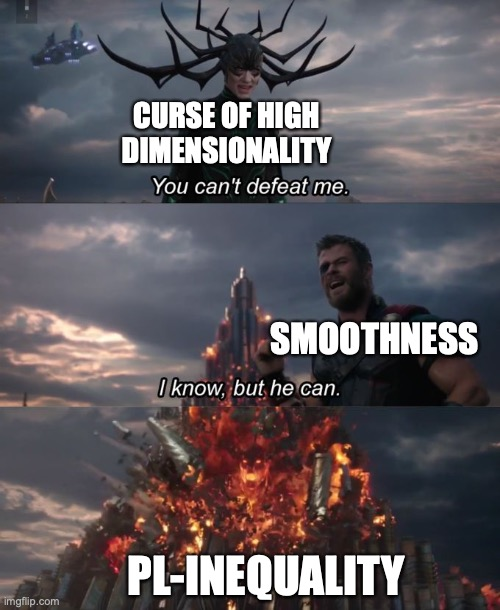
\includegraphics[scale=0.4]{50wuxh.jpg}
    \caption{A quality meme}
\end{figure}
\subsubsection{GD with Smooth Functions satisfying PL-inequality}
Now, using this PL-inequality, we will show that we can establish the following convergence rate:
\begin{mdframed}
\begin{theorem}
For a smooth function $f: \R^d \to \R$ which also satisfies the PL-inequality, for any $\epsilon > 0$ the following convergence criterion can be met in $\O(\log(1/\epsilon))$ iterations:
\begin{align*}
    f(w_t) - f^* \leq \epsilon
\end{align*}
\end{theorem}
\end{mdframed}

\begin{proof}
 Assuming smoothness of our function we were able to derive the following bound in the proof of \autoref{gd:thm:smooth:convg}
\begin{align*}
f \lp w_{t+1} \rp \leq f \lp w_t \rp - \frac{1}{2L} \norm{\grad f \lp w_t \rp }^2
\end{align*}
Under the PL-inequality (\autoref{gd:defn:pl}) we have
\begin{align*}
    -\norm{\grad f(w_t)}^2 \leq -2\mu \lp f(w_t) - f^*) \rp
\end{align*}
and thus,
\begin{align*}
    f(w_{t+1}) \leq f(w_t) - \frac{\mu}{L} \lp f(w_t) - f^* \rp \\
    f(w_{t+1}) - f^* \leq (f(w_t) - f^*) - \frac{\mu}{L} \lp f(w_t) - f^* \rp \\
    f(w_{t+1}) - f^* \leq \lp 1 - \frac{\mu}{L} \rp \lp f(w_t) - f^*) \rp \leq \lp 1 - \frac{\mu}{L}\rp^t (f(w_0) - f^*)
\end{align*}
Finally, observe that
\begin{align*}
    1 + x \leq e^x
\end{align*}
Thus
\begin{align*}
    f(w_{t+1}) - f^* \leq \exp\lp-\frac{\mu}{L} \cdot t\rp \left[f(w_0) - f^*\right]
\end{align*}
Hence, we have $f(w_t) - f^* \leq \epsilon$ for any $t$ satisfying
\begin{align*}
    t \geq \frac{L}{\mu} \log{(f(w_0) - f^*) / \epsilon)} = \O(\log(1/\epsilon))
\end{align*}
\end{proof}

\subsubsection{Properties of the PL-inequality}
The PL-inequality is general enough that it is satisfied by many standard convex models. However, it has the additional benefit of being satisfied even by some non-convex functions like $w^2 + 3\sin^2(w)$. It is also satisfied for many classes of {\em overparameterized} neural networks \cite{liu2020toward}, and is the reason for good empirical performance of GD in optimizing neural networks.

\subsubsection{Strong Convexity and PL-inequality}
Strong convexity, as the name may imply, is a stronger variant of convexity which induces some nice properties.
\begin{defn}[Strong Convexity]
A function is $\mu$-strongly convex if the following function is convex:
\begin{align*}
    f(w) - \frac{mu}{2}\norm{w}^2
\end{align*}

If $f$ is $C^2$, then equivalently
\begin{align*}
    \grad^2 f(w) \succcurlyeq \mu I
\end{align*}
\end{defn}
\begin{prop}
If $f: \R^d \to \R$ is a $\mu$-strongly convex function, then
\begin{enumerate}
    \item A {\em unique} minimizer exists
    \item if $f$ is additionally $C^1$, then it satisfies the PL inequality.
\end{enumerate}
\end{prop}
If we have a convex loss function $f$, then adding $\ell_2$-regularization makes it strongly convex. This can improve the convergence rate from $\O(1/t)$ to exponential. This motivates the weight-decay regularization technique used for neural networks.

\subsection{Stochastic Gradient Descent}
Until now, we have been talking about gradient descent while somewhat closing our eyes towards the reality of computational cost. Unfortunately,
for large datasets computing the gradient across all of our training samples is quite intractable. The cost of each gradient descent update scales linearly
with both (1) the number of variables, and (2) the number of training samples. Thus, in order to make the problem tractable we instead consider
a randomized version of GD, {\em Stochastic Gradient Descent} (SGD).

SGD performs pretty much the same update as vanilla gradient descent with the modification that instead of computing the gradient across all
training samples, we will simply compute the gradient with respect to a {\em randomly} chosen sample. In practice, the random choice will be without replacement
,however, to simplify mathematical analysis we will always assume it is with replacement. 
        \begin{algorithm}[H]
        \caption{Stochastic Gradient Descent Psuedocode}
        \label{algo:sgd}
        \begin{algorithmic}[1]
        \Procedure{StochasticGradientDescent}{$f, \eta$}
        \State Initialize $x_0 \in_R \R^d$
        \While{not converged}
            \State pick $j_t \in_R [n]$
            \State $x_{t+1} = x_t - \eta \grad f_{j_t}(x_t)$
        \EndWhile
        \Return $x_{t+1}$
        \EndProcedure
        \end{algorithmic}
        \end{algorithm}
The reader may constrast \autoref{algo:gd} with \autoref{algo:sgd}. Note that here we assume the loss function $f$ is of the form
\begin{align*}
    f(w_t) = \frac{1}{n} \sum_{i = 1}^n f_i(w)
\end{align*}
Where $f_i$ is the loss with respect to the $i^{\text{th}}$ training example. Observe with SGD we shave off a factor of $n$ in the time spent
on each gradient update. Moreover, the SGD vector also enjoys the following nice property:
\begin{prop}
    The stocastic gradient vector is an {\em unbiased} estimate of the full gradient. i.e.,
    \begin{align*}
        \E\left[\grad f_{j_t}(w)\right] = \frac{1}{n} \sum_{j = 1}^n \grad f_j(w) = \grad f(w)
    \end{align*}
\end{prop}
When implementing SGD, $x_0$ is generally sampled as an i.i.d Gaussian vector. While SGD sounds great right now, it does have
(at least) two challenges:
\begin{enumerate}
    \item It takes $n$ iterations before the model has ``seen'' all the training data.
    \item The individual updates may be more noisy.
\end{enumerate}
Thus, as with many things in life, a solution which is often used in practice is {\bf Mini-Batching}.
In mini-batching, instead of just selecting $1$ random component of the loss function, we pick a batch size $B$, and
pick a random batch of $B$ components, and compute the average gradient with respect to the batch. Thus, the update becomes
\begin{algorithm}[H]
    \caption{Mini-Batch Stochastic Gradient Descent Psuedocode}
    \label{algo:mini_batch_sgd}
    \begin{algorithmic}[1]
    \Procedure{MinibatchStochasticGradientDescent}{$f, \eta, B$}
    \State Initialize $x_0 \in_R \R^d$
    \While{not converged}
        \State pick $S \subset [n]$ where $|S| = B$
        \State $x_{t+1} = x_t - \eta \frac{1}{B} \sum_{j \in S} \grad f_{j}(x_t)$
    \EndWhile
    \Return $x_{t+1}$
    \EndProcedure
    \end{algorithmic}
    \end{algorithm}
Observe that by linearity of expectation this is still an unbiased estimate of the full gradient vector.
However, we have now reduced the variance. In particular, observe
\begin{align*}
    \Var\lp \frac{1}{B} \sum_{j \in S} \grad f_j(x_t) \rp = \sum_{j \in S} \Var \lp \frac{1}{B}\grad f_j(x_t) \rp = B \cdot \frac{1}{B^2} \Var \lp f_1(x_t) \rp = \frac{1}{B} \Var \lp f_1(x_t) \rp
\end{align*}
It is advisable to pick a reasonable batch-size based on available hardware. For instance, it may be a good idea to make sure your batch fits
in your GPU memory, or perhaps isn't too large with respect to the bandwidth/throughput of the memory bus between CPU and GPU memory etc. 
Ok, that's all great, but what about convergence? With minibatching we seem to have gotten something which is on expectation the full gradient, and
with {\em lower} variance than just SGD, but does that mean the same guarantees from prior sections carry over? Not quite.

\begin{theorem}
    Suppose we are optimizing a loss function $f(w) = \frac{1}{n} \sum_{j = 1}^n f_j(w)$ where the following are satisfied:
    \begin{enumerate}
        \item Each $f_j$ is $L$-Lipschitz smooth ($\norm{\grad f_j(u) - \grad f_j(v)}_2 \leq L \norm{u - v}_2)$
        \item Each $f_j$ is convex
        \item The total loss $f$ is $\mu$-strongly convex
        \item At the minimizing solution $w_*$ the ``component noise'' is $\sigma^2 = \frac{1}{n} \sum_{j = 1}^n \norm{\grad f_j(w_*)}^2$
    \end{enumerate}
    Then, assuming step-size $\alpha \leq \frac{1}{L}$ we have
    \begin{align*}
        \E\left[ \norm{w_t - w_*}_2^2 \right] \leq \left(1 - 2\alpha\mu\left(1 - \alpha L\right)^t\right) \norm{w_0 - w_*}_2^2 + \alpha \frac{\sigma^2}{\mu \left(1 - \alpha L\right)}
    \end{align*}
\end{theorem}

% TODO: add commentary on the shape / intuition for this inequality
% from lecture
